\cleardoublepage
\chapter{User Interface}
\label{ch:2}

%------------------------------------------------
\section{Parameter Window}

\begin{fullwidth}

The 'Parameter Window' is where all an Operator's parameters can be accessed.

There are two ways to access the 'Parameter Window'. The first is using the 'P' key. This will open a docked 'Parameter Window' in the top-right hand corner of the pane. This docked 'Parameter Window' will display the parameters of whatever Operator is selected.

The second way to access the 'Parameter Window' is by right clicking on an Operator and selecting 'Parameters...'. This will open up a floating 'Parameter Window' for the Operator. This method differs from the first in that the parameters will not change if another Operator is selected. This is useful for being able to manage the parameters of multiple Operators simultaneously.

Every Operator has a different set of parameters, but all 'Parameter Windows' have the same set of options. Below is a diagram highlighting the options:

\begin{center}
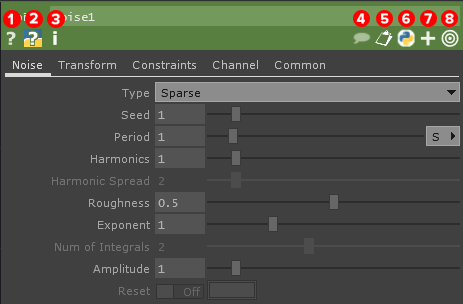
\includegraphics[width=13cm]{./img/2.1/parameter-window.png}
\end{center}

From left to right, the options are as follows:

\begin{enumerate}
\item Operator Help: opens the Operator's Wiki help page in a new browser window
\item Operator Python Help: opens the Operator's Python Wiki help page in a new browser
\item Operator Information Dialog: displays information about the Operator's process, similar to middle-clicking an Operator
\item Comment: display and edit Operator comments
\item Copied Parameters: displays parameters copied via the right click menu
\item Language: choose whether the Operator will use Python or tscript as its scripting language
\item Expand/Collapse Parameters: expand or collapse all the Operator's parameters
\item Non-default Parameters: display only parameters that have been changed from their default values
\end{enumerate}

\end{fullwidth}
%------------------------------------------------
\section{Parameters}

\begin{fullwidth}

Parameters can be entered in a number of ways. Depending on the situation, some parameters may require a static value, and some may need to be driven by other values and inputs. Each parameter has three modes. Each mode is quite different and each defines how the parameter behaves. The three modes are:

\begin{enumerate}
\item Constant mode
\item Expression mode
\item Export mode
\end{enumerate}

Constant mode is the default for most parameters, and is represented by a grey colour scheme in the value field. Expression mode is used for Python, tscript, or mathematical operations and scripts. Expression mode is represented by a dark grey and light blue colour scheme. Export mode is used to directly reference CHOP channels.  It is represented by a light green colour scheme.

Each of an Operators parameters can be independently changed between the three modes. To change the mode of a parameter, hover the mouse over the parameter's name. A '+' sign will appear near the parameter's name, similarly to the diagram below.

\begin{center}
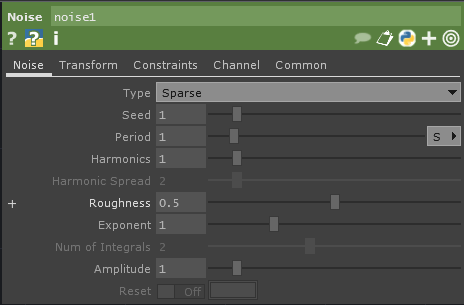
\includegraphics[width=12cm]{./img/2.2/parameters-1.PNG}
\end{center}

Once hovering over the parameter's name, click it and it will expand, displaying more information and options, similarly to the diagram below:

\begin{center}
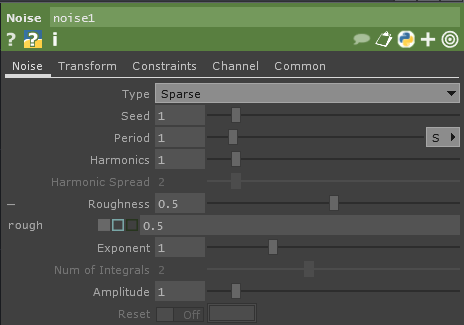
\includegraphics[width=12cm]{./img/2.2/parameters-2.PNG} 
\end{center}

There are three main elements that are available once a parameter is expanded. The first on the left, is the parameter's scripting name. This scripting name is needed whenever that parameter is referenced in any of TouchDesigner's scripting languages. In the above diagram, the scripting name for the Noise CHOP's Roughness is 'rough'. Continuing the above example, the Python script to set the Roughness of the above Noise CHOP to '1' would be:

\begin{lstlisting}
op('noise').par.rough = 1
\end{lstlisting}

The second element is the three coloured squares. These squares represent the different modes for the parameter, as discussed above. Operator parameters set to Constant mode are represented by a filled grey square. This parameter can be changed to Expression mode by clicking on the outline of the light blue square. Once clicked, the light blue square will be filled, and the value field to the right will also be coloured to reflect the parameter's mode.

\begin{center}
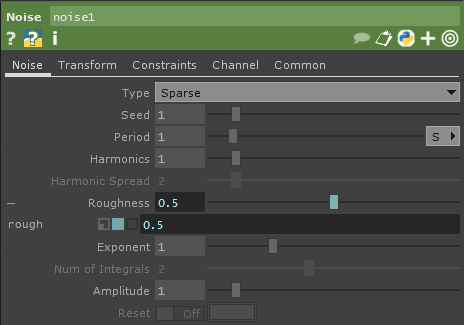
\includegraphics[width=12cm]{./img/2.2/parameters-3.PNG}
\end{center}

To change the parameter's mode to Export mode, a CHOP channel needs to be dragged and dropped on the parameter, at which point it will take up Export mode's colour scheme, and the green box will be filled in.

\begin{center}
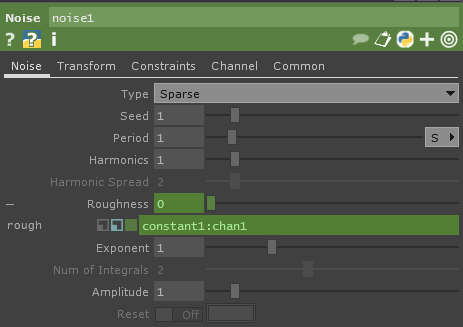
\includegraphics[width=12cm]{./img/2.2/parameters-4.PNG}
\end{center}

The third element of the expanded parameter is the value field. The value field displays a different piece of information depending on the parameter mode. In Constant mode, the value field displays the current value, and can be edited by clicking and typing in the field. In Expression mode, the value field displays the script of Python or tscript that is being evaluated. The expression can be edited by clicking and typing in the value field. In Export mode, the value field displays two pieces of information separated by a colon. The text before the colon displays the path of the CHOP that is exporting to this parameter. The text after the colon is the name of the channel being exported from the CHOP. Because these values are being imposed by another Operator, the value field cannot be edited while the parameter is in Export mode.

\end{fullwidth}
%------------------------------------------------
\section{Transport Controls}

\begin{fullwidth}

The transport bar functions similarly to the transport bars of many other applications. To go through it quickly, from left to right the buttons do the following:

\begin{center}
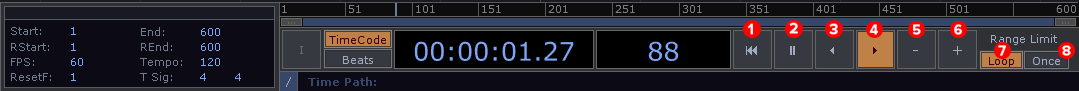
\includegraphics{./img/2.3/transport-1.png}
\end{center}

\begin{enumerate}
\item Resets timeline to frame 1
\item Pause the timeline
\item Play timeline in reverse
\item Play timeline forward
\item Step one frame backward
\item Step one frame forward
\item Setting 'Range Limit' to 'Loop' will continuously loop the timeline
\item Setting 'Range Limit' to 'Once' will play through the timeline and hold the last frame
\end{enumerate}

The most used functions of the timeline are 'Play' and 'Pause', which can be accessed quickly by pressing the 'Space bar' on the keyboard.

\end{fullwidth}
%------------------------------------------------
\section{Timeline Settings}

\begin{fullwidth}

Unless media or animations is locked to the timeline, the 'Timeline settings' won't need to be regularly accessed. The 'Timeline settings' can be found in the bottom left of the window. The key things to know about this area are that the project's 'FPS' and 'Tempo' can be changed here. The project's 'FPS' determines the rate at which the project will render frames. By default it is set to 60 FPS, meaning that it TouchDesigner will try to render 60 frames every second. The 'Tempo' will set the BPM (beats per minute) of the project, for use by the Beat CHOP. 

The 'Timeline settings' are use more in situations where animations and media need to be locked to a consistent timeline. The frame controls include 'Start' and 'End', which control the start frame and end frame of the timeline, as well as 'RStart' and 'REnd', which control the loop start and loop end of the timeline. With these settings, it is possible to create an animation that spans the entire timeline, which could be 4000 frames, while still leaving the option to loop a small section of the timeline to work within. 

\begin{center}
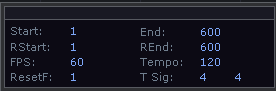
\includegraphics[width=8cm]{./img/2.4/timeline.png}
\end{center}

\end{fullwidth}
%------------------------------------------------
\section{Panes}

\begin{fullwidth}

Using panes regularly can save a ton of time when moving back and forth between Networks. Having to travel through 3 Networks to change a parameter, only to have to travel back to see then changes is a waste of time. Panes take the current window, split it horizontally or vertically as many times as desired. Each pane layout can be saved for later use. 

\begin{center}
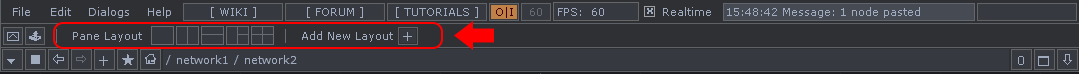
\includegraphics{./img/2.5/panes-1.png}
\end{center}

The diagram above highlights the pane presets that are available by default. The presets provide quick access to a few standard configurations of panes including split left and right, split top and bottom, a 3 pane setup, and a 4 pane setup. Saving pane presets is as easy as clicking the 'Add New Layout +' button, entering a name, and clicking 'Ok'. Saving a layout not only saves the size and position of the panes, but also saves each pane's type. See the diagram below highlights interesting pane layouts that are possible.

\begin{center}
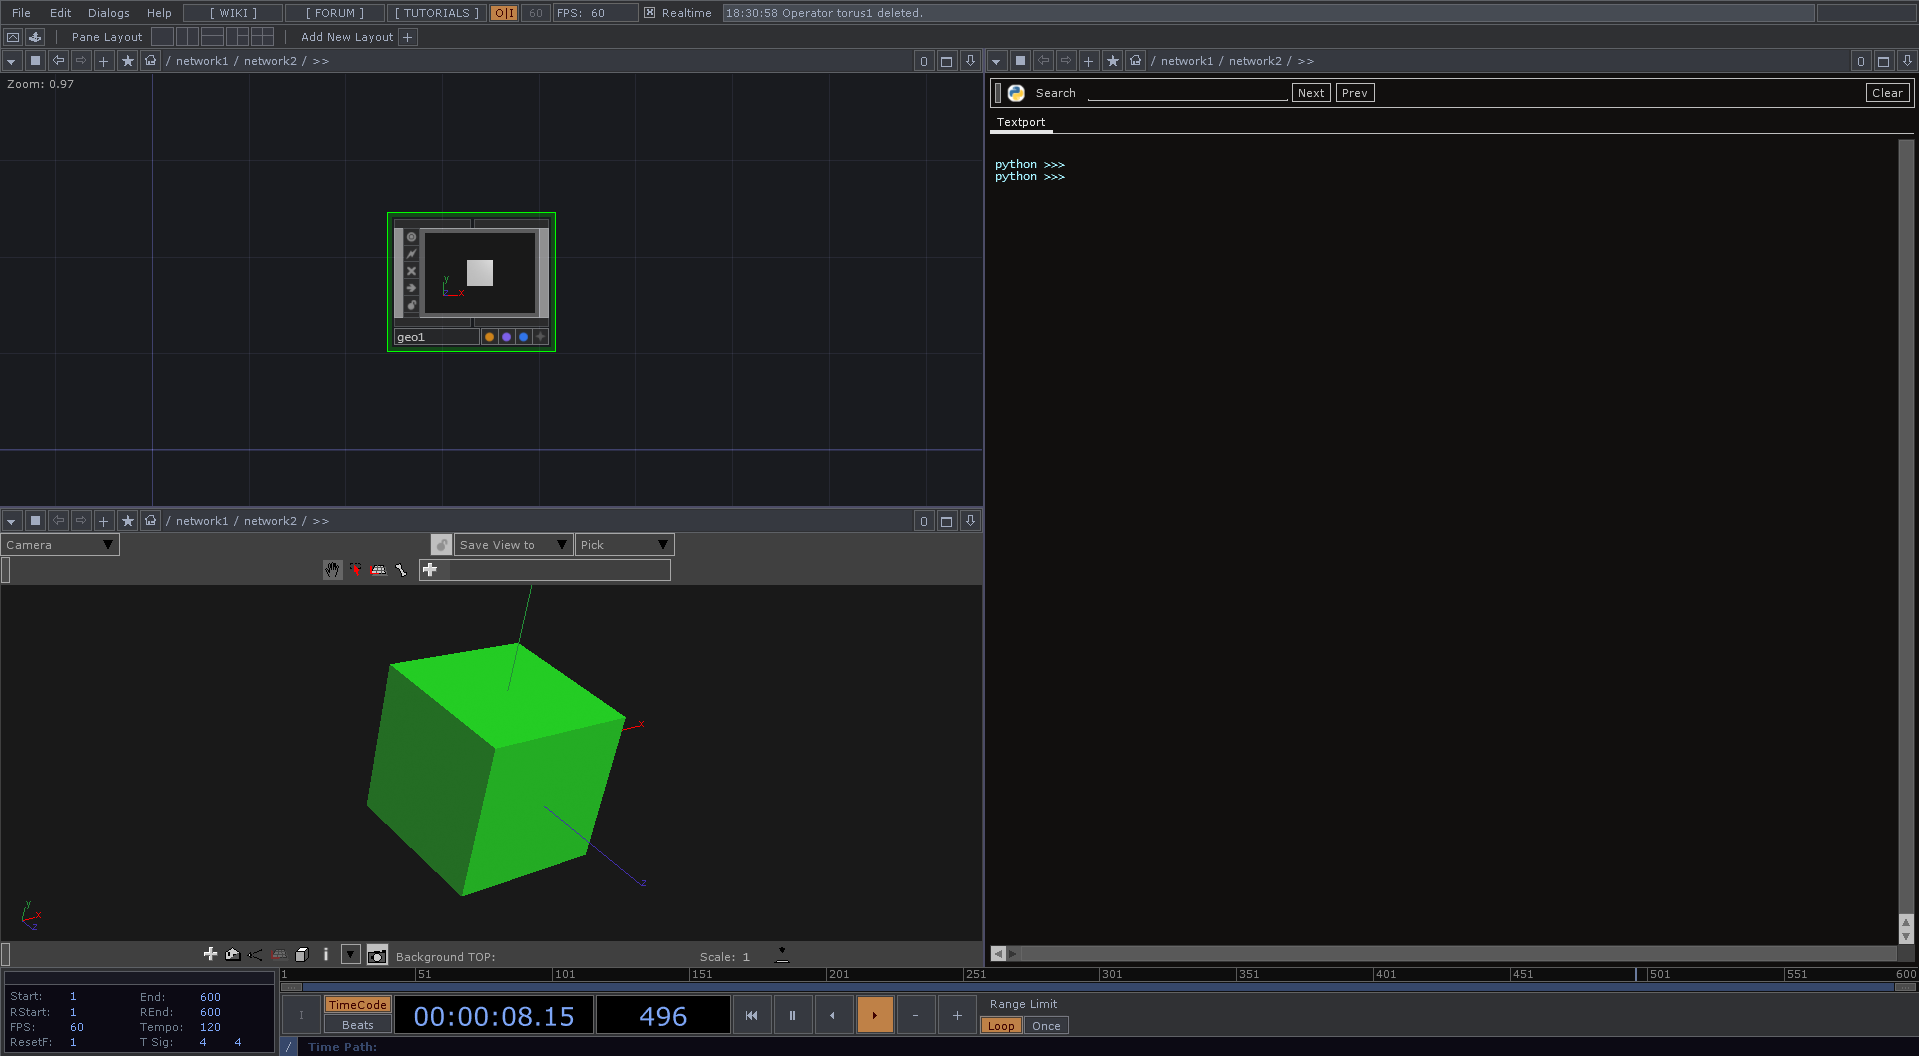
\includegraphics{./img/2.5/panes-2.png}
\end{center}

Panes are be able to display unique types of content, whether they are other dialogues, Networks, or viewers. Being able to mix and match combinations of viewers and Network editors allows for a lot of flexibility. In the diagram above, the top left pane is a Network editor. On the right-hand side, is a Textport, and on the bottom-left, there is a Geometry Viewer. Again, saving this layout would not only save the pane arrangement, but also the pane types. This is useful when working on a project with a lot of different elements, where jumping between something like the setup above, and a simple Network editor, can save quite a bit of time in the long run.

The keyboard shortcuts for working with panes are as follows:

\begin{itemize}
\item Alt + [ : Vertically split current pane under mouse
\item Alt + ] : Horizontally split current pane under mouse
\item Alt + Z : close pane under mouse
\end{itemize}

\end{fullwidth}
%------------------------------------------------
\section{Palette Browser}

\begin{fullwidth}

The Palette Browser can be thought of as a component library. The Palette Browser holds '.tox' files (or TouchDesigner Component files). These files contain a single Component Operator, that can hold a Network of other Operators. This means that a series of frequently used Operators, UI components, Python scripts, and more, can be created inside of a single Component Operator, saved as a '.tox' file, and quickly accessed at any time in the future.

Open the Palette Browser, and look through the large number of pre-existing '.tox' files that are available. To open the Palette Browser, use the keyboard command 'Alt + L'. Blank projects start with the Palette Browser open by default, and docked to the left side of the window. Let's try one of the pre-built components. 

Under the 'Derivative' section, navigate to 'Tools', and then finally drag and drop the 'Blend' component into a new project. Looking at the 'Blend' component's UI, it is clear that there is quite a bit going on inside. Before diving deeper, take a moment to connect two inputs and try the 'Blend' component. Activate the viewer, click on the button underneath the image to select a blend mode, and then drag the semi-transparent handle across the image to blend between the inputs. This is a useful tool, and all it took was a simple drag and drop from the Palette Browser!

One of the goals of this book is to create some tools that can be added to the Palette Browser, so that they may be used regularly. There are two ways to add a component to the Palette Browser. The first is a drag and drop method. To do so, select 'My Components' from the top portion of the browser. Then drag any component from the Network and drop it into the lower portion of the Palette Browser. It will then be added to 'My Components' repository. The second method of adding a component is to drag s saved '.tox' file from Windows Explorer, and drop it in the same region mentioned above. The diagram below illustrates exactly where components should be dropped.  

\begin{center}
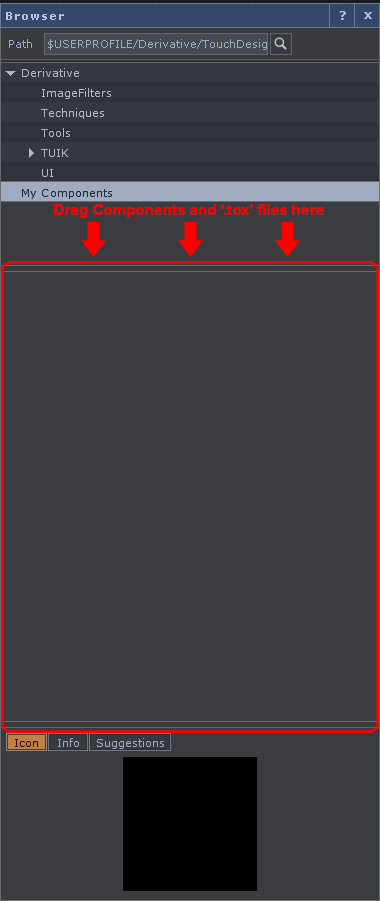
\includegraphics[width=6cm]{./img/2.6/palette-1.png}
\end{center}

\end{fullwidth}
%------------------------------------------------
\section{Search Dialog}

\begin{fullwidth}

The 'Search Dialog' is incredibly helpful as projects become more complicated, and riddled with Python scripts and nested Networks. The 'Search Dialog' can find a multitude of things in a multitude of places, and searches can be as broad, or specific, as needed. It is accessible in the 'Edit' menu at the top of  the screen, or by pressing 'F3' on the keyboard.

The 'Basic' search can not only find Operators, but can search through Python code. Frequently, Python is used to change Operator parameters based on input sources. Sometimes, in the thick of Python scripts, it is easy to lose track of specific lines of code. A quick search for the code below will return a list of every single line of code that involves changing parameters of the Operators with 'transform' in their name:

\begin{lstlisting}
op('transform').par
\end{lstlisting}

Sifting through the results is much easier than manually looking through Networks full of code. 


The 'Advanced' search can search by any combination of name, Operator type, comments, flags, and more. When returning to past projects, sometimes it takes some time to relocate and reacclimatize to the inner workings of complex logic systems. In this stretch of time, searching for operators by vague name and type can save a ton of time. For example, in an extremely nested system, somewhere in the depths of it might be a Movie In TOP that has the word 'movie' in its name. These little pieces of information about the Operator type, and partial name, can be used to create a fairly precise search. 

When a search has yielded results, each result can be double clicked on to open the Network in a new floating pane. Here, the results can be can quickly previewed, and simple changes can be made within this pane, without affecting the current work area.

\end{fullwidth}
%------------------------------------------------
\section{Realtime Flag}

\begin{fullwidth}

\begin{center}
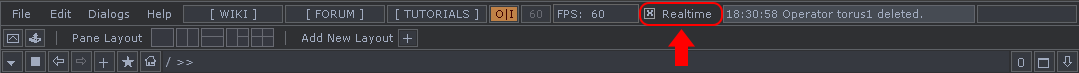
\includegraphics{./img/2.8/realtime-1.png}
\end{center}

The Realtime flag changes TouchDesigner's behaviour significantly. When it is active (it is active by default), TouchDesigner will always prioritize real-world time. In a simple example, if a movie file is 30 seconds long, no matter what happens, TouchDesigner will try to play it over the course of 30 seconds. If this means that frames need to be dropped, TouchDesigner will try to honour time. This is the mode used for most real-time installation and performance work. 

When the Realtime flag is off, TouchDesigner will prioritize frame rendering over real-world time. In the example mentioned above, if Realtime is off, TouchDesigner would take as long as it needed to process and render each frame, falling out of real-world time to display every frame. This mode is useful when exporting complex animations or 3D renderings. Imagine this mode to be a close to real-time version of rendering out of Adobe After Effects. 


\end{fullwidth}
%------------------------------------------------
\section{Useful Shortcuts}

\begin{fullwidth}

Below is a bullet point list of some useful shortcuts:

\vspace{3mm}

\noindent When hovering over the Network:
\begin{itemize}
\item 'P' - Opens and closes the selected Operator's Parameter window
\item 'O' - Opens and closes a visual overview of the Network in the bottom-left corner of the pane
\item 'C' - Opens and closes the Colour Palette. This can add a coloured outline to the selected Operators for easier identification
\end{itemize}

\vspace{3mm}

\noindent With an Operator selected:
\begin{itemize}
\item 'A' - Allows interaction with the Operator's viewer
\item 'B' - Bypass and un-bypass the selected Operator
\item 'H' - Performs the 'Home All' action on the Network, which is the equivalent to fitting all Operators of a Network onto the screen 
\item 'R' - Toggles the Operator's Render Flag (if it has one)
\item 'D' - Toggles the Operator's Display Flag (if it has one)
\end{itemize}

\vspace{3mm}

\noindent After selecting one or more Operators:
\begin{itemize}
\item 'Control + C' - Copy selected Operators
\item 'Control + V' - Paste copied Operators
\item 'Control + Shift + V' - Paste copied Operators at the mouse
\end{itemize}

\end{fullwidth}
%------------------------------------------------